\subsubsection{Electronic design}
In this project, the user interface is implemented in the form of an android application. Commands are communicated to a microcontroller via a serial connection with a Bluetooth module. The microcontroller does all of the calculations and performs the necessary algorithms to determine what should be done with which servo and then communicates this to the relevant servo motor. The algorithm for movement also takes some inputs from the microcontroller into account.\\

The electronics to be implemented for this project is listed below. 
\begin{itemize}
\item Power regulation and supply.
\item Support electronics for the microcontroller.
\item Digital input signal conditioning.
\item Bluetooth module interfacing.
\item Digital output driving where applicable.
\item Servo power control switch
\end{itemize}
Each of these items are discussed separately below.\\

Power regulation and supply for the project can be divided into two parts. The first of these is the low voltage, low power part that supplies the microcontroller, Bluetooth module and support electronics. The second part is the higher voltage, high power part that supplies power exclusively to the servo motors. Both these supplies will be powered by Li-Ion 18650 cells because of their high power density. The nominal voltage of these cells are $3.7V$. The low voltage, low power supply can easily be powered from a single cell making use of a low dropout (LDO) linear regulator to provide the $3.3V$ rail required. A linear voltage regulator is not suited for the high power application, mainly for two reasons. The first of the two is that these regulators are rarely rated for use above $1.5A$. The second is that a linear regulator dissipates power in itself as heat in order to regulate voltage. This means that the voltage drop formed over the device to bring the output voltage down is dissipated in the device. The power dissipated can be quantified by

\begin{align}
P &= V\times I\\
&= (V_{in}-V_{out})\times I
\end{align}

This is fine for low current applications but sufficient cooling quickly becomes a problem at currents in the Ampere range.
A better solution for regulation at high power is making use of a step-down DC-DC converter. The efficiency of this topology is much greater than for linear regulators. Most are in excess of $90\%$ if operated within the design limits. Since DC-DC converters can become very complex and it is far outside the scope of this project, a complete off-the-shelf module was implemented instead of designing and building one from first principles. Figure \ref{fig:PowerSupply} shows the power supply layout for the robot.

\begin{figure}[H]
\centering
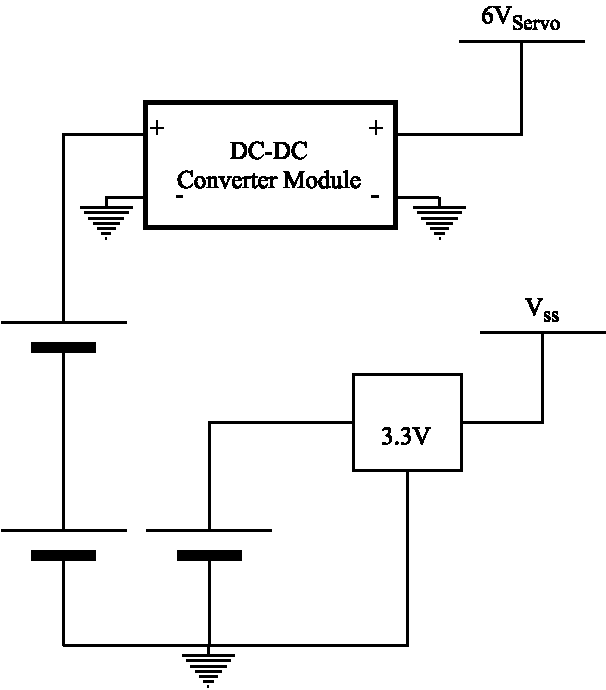
\includegraphics[scale = 1]{pics/PowerSupply.pdf}
\caption{Diagram showing the power supply layout for the robot.}
\label{fig:PowerSupply}
\end{figure}

The support electronics for the microcontroller includes everything necessary for it to be able to start after power up and function normally. The application note provided by the manufacturer has detailed instructions and schematics on this and it was implemented as recommended for this project. This includes ceramic capacitors on all of the power supply pins, electrolytic capacitors on the power rails, a high frequency crystal oscillator, timing capacitors, a reset switch, various pull-up and pull-down resistors and a selector for pulling the BOOT pin high or low. More details on this can be fond in the technical documentation section of the report.\\

In order to protect digital input pins on the microcontroller, as well as debouncing input signals from switches, a small interface circuit is used between an input and a digital pin. This is implemented from prior knowledge gained in earlier modules. Figure \ref{fig:InputProtection} shows the schematic for this.

\begin{figure}[H]
\centering
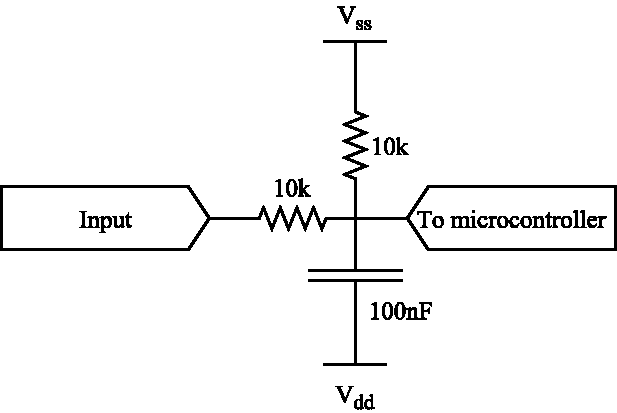
\includegraphics[scale = 1]{pics/InputProtection.pdf}
\caption{Diagram showing the digital input protection circuit for the robot.}
\label{fig:InputProtection}
\end{figure}

The Bluetooth module used in this project does all of the Bluetooth protocol and decryption automatically and makes the data available through the serial interface. This means that the module is powered by the rails of the microcontroller and all that is further required to receive information is to connect the $TX$ pin of the module to the \textit{USART\_RX} pin of the microcontroller.\\

In order to make the actions and decisions of the robot more apparent to the user, a red, green and blue (RGB) LED array is connected to the microcontroller. Different colours can then be used to indicate different states of the robot. Since the LEDs can't be powered directly from a digital output pin, a driver will have to be built to protect both the microcontroller and the LEDs. Figure \ref{fig:LEDDriver} shows the schematic for this. Each LED requires a bipolar junction transistor (BJT) of type PNP. The PNP is required because the RGB LED has a common ground and therefore has to be switched on the positive side. The microcontroller is used to pull the base of the PNP  high or low. The LED will then switch off or on respectively.

\begin{figure}[H]
\centering
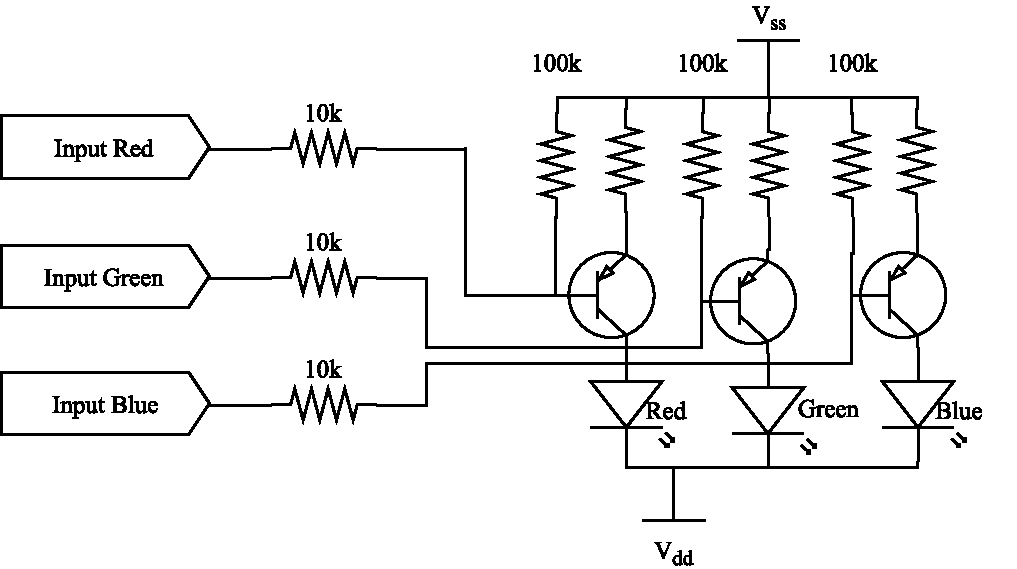
\includegraphics[scale = 1]{pics/LEDDriver.pdf}
\caption{Diagram showing the driver circuit for the RGB LED array.}
\label{fig:LEDDriver}
\end{figure}

Servo motors constantly use power to hold the position they are in. When the robot is idle, waiting for a Bluetooth connection, it is unnecessary for the servo motors to be consuming current. The circuit illustrated in Figure \ref{fig:PowerSwitch}  is designed to switch power to a rail dedicated to servo motor supply. It uses a P-channel MOSFET as well as a NPN BJT. The P-channel MOSFET is required to switch the positive rail with a low internal power dissipation due to a low drain-source resistance when switched on. The BJT is necessary to switch it on because the microcontroller pin on its own can't reach the 6V required to completely switch off. When the pin is low, the BJT is switched off, the MOSFET gate is pulled high by the resistor and therefore the MOSFET is off. When the pin is high, the BJT pulls the MOSFET gate low and the MOSFET is fully on, thereby turning the servo rail on.

\begin{figure}[H]
\centering
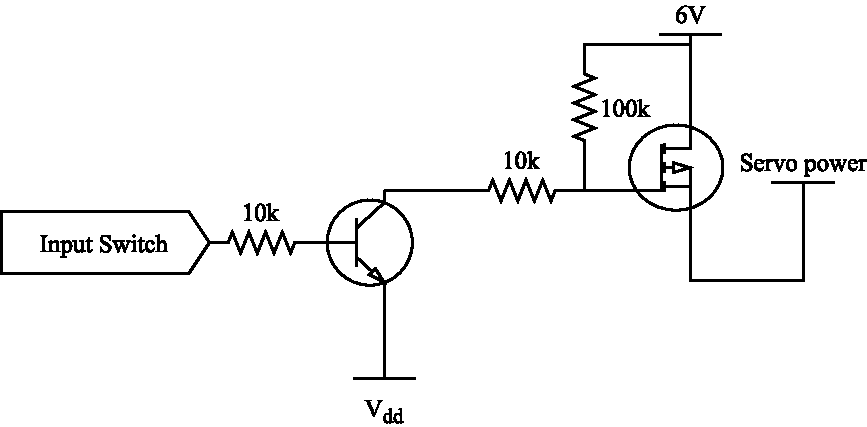
\includegraphics[scale = 1]{pics/PowerSwitch.pdf}
\caption{Diagram showing the driver circuit for the RGB LED array.}
\label{fig:PowerSwitch}
\end{figure}

\subsubsection{Electronic implementation}

The microcontroller chosen is an STM32F576GTV6. This specific model was chosen because of its powerful FPU, high clock speed and the large pin count for possible expanding later. This unit is, however, only available in an LQFP100 package with 0.4mm pin spacing. This was soldered to a breakout board to make interfacing with the hardware easier. The breakout board was glued to a Veroboard where the rest of the electronics, discussed above, was implemented.